\documentclass{article}

% if you need to pass options to natbib, use, e.g.:
% \PassOptionsToPackage{numbers, compress}{natbib}
% before loading nips_2016
%
% to avoid loading the natbib package, add option nonatbib:
% \usepackage[nonatbib]{nips_2016}

\usepackage[final, nonatbib]{nips_2016}

% to compile a camera-ready version, add the [final] option, e.g.:
%\usepackage[final]{nips_2016}

\usepackage[utf8]{inputenc} % allow utf-8 input
\usepackage[T1]{fontenc}    % use 8-bit T1 fonts
\usepackage{hyperref}       % hyperlinks
\usepackage{url}            % simple URL typesetting
\usepackage{booktabs}       % professional-quality tables
\usepackage{amsfonts}       % blackboard math symbols
\usepackage{nicefrac}       % compact symbols for 1/2, etc.
\usepackage{microtype}      % microtypography

% My packages
\usepackage{amsmath}        %Matrix
\usepackage{graphicx}       %Graphics
\usepackage{subcaption}     %Subfigures


\title{Design Optimization of a Stochastic Multi-Objective Problem: \\Gaussian Process Regressions for Objective Surrogates}

% The \author macro works with any number of authors. There are two
% commands used to separate the names and addresses of multiple
% authors: \And and \AND.
%
% Using \And between authors leaves it to LaTeX to determine where to
% break the lines. Using \AND forces a line break at that point. So,
% if LaTeX puts 3 of 4 authors names on the first line, and the last
% on the second line, try using \AND instead of \And before the third
% author name.

\author{
  Juan S. Martinez\\
  Department of Electrical and Electronic Engineering\\
  Universidad de los Andes\\
  Bogotá, Colombia \\
  \texttt{js.martinez777@uniandes.edu.co} \\
  \And
  Piyush Pandita \\
  School of Mechanical Engineering \\
  Purdue University \\
  West Lafayette, Indiana 47907\\
  \texttt{ppandit@purdue.edu} \\
  \AND
  Ilias Bilionis \\
  School of Mechanical Engineering \\
  Purdue University \\
  West Lafayette, Indiana 47907\\
  \texttt{ibilion@purdue.edu} \\
  \And
  Rohit K. Tripathy \\
  School of Mechanical Engineering \\
  Purdue University \\
  West Lafayette, Indiana 47907\\
  \texttt{rtripath@purdue.edu} \\
  %% \And
  %% Coauthor \\
  %% Affiliation \\
  %% Address \\
  %% \texttt{email} \\
}

\begin{document}
% \nipsfinalcopy is no longer used

\maketitle

\begin{abstract}
    Multi-objective optimization (MOO) problems arise frequently in science and engineering situations, where a set of multiple quantities of interest (QoI) of a certain system are to be maximized or minimized. The objective of the optimization problem is to find the set of input parameters that generate the set of optimal outputs, mathematically known as the Pareto front. Solving the MOO problem is a challenge for many applications where complex systems are to be optimized, as expensive experiments can be performed only a constrained number of times and there is a limited set of data to work with, e.g, a roll-to-roll microwave plasma chemical vapor deposition (MPCVD) reactor for manufacturing high quality graphene. For this purpose, the current MOO techniques, e.g, evolutionary algorithms, particle swarm optimization, require a large amount of observations and are not applicable. On the other hand, recent extensions of Bayesian global optimization (BGO) are able to tackle the problem, replacing expensive objective functions with surrogates trained with few input-output pairs that are cheap to evaluate. This probabilistic surrogates provide prediction error bars that correspond to the epistemic uncertainty induced by limited data, which quantify the improvement that a hypothetical experiment could contribute to the state of knowledge of the Pareto front in the MOO problem, in order to sequentially select the designs that maximize this enhancement. This work presents the development of a NanoHUB tool that enables experimentalists to use this methodology and the results of its usage with a synthetic example and the MPCVD case.
\end{abstract}

\section{Introduction}

A great variety of problems in science and engineering can be expressed as optimization problems, where a function that describes the operation of a system should be minimized or maximized, restricted to some constraints imposed by the system itself. For example, a supermarket may want to minimize its inventory purchases while keeping enough stock for its operation, or in a metal-forming shop, a manufacturer may want to maximize the performance of the manufacturing system adjusting certain parameters, like the forming temperature and the die geometry \cite{Huang2006}. Moreover, real optimization problems do not have trivial solutions, since in many cases the optimization could target: black-box systems where the physics and mathematics of the process are not well known; expensive simulations or evaluations of objective functions \cite{Jones1998}; introduction of uncertainty at the output due to noise in the input data; and multiple objectives. In this context, a need for the design of a method for solving stochastic multi-objective optimization problems arises and becomes important in the science and engineering community.

A typical problem in experimental research is to determine the parameters of an experiment that can maximize or minimize some output quantity. There could be inadequate knowledge of the physics of the underlying problem. The experiment may also be expensive (computationally or financially) and thus may only be performed  a limited number of times under a finite budget. Such problems are well suited to be treated as Bayesian global optimization problems where limited output observations are used to build a model that could describe the system with the highest accuracy possible. Optimization under these circumstances has been approached from different perspectives, for example, advances in efficient global optimization of expensive simulations have been made through the analysis of various criteria of the problem, like the expected improvement (EI) of running the simulation at a particular point; also, stopping criteria for the sequential optimization processes that rules black-box problems have also been developed \cite{Jones1998}, as well as curiosity-driven techniques \cite{Schaul2011}. In this matter, the structure for solving black-box optimization problems is based on building response surfaces over observed data. The taxonomy of this process includes the use of different criteria to evaluate the sequential process of optimization, in which the EI information acquisition scheme has proven to be more efficient than any other criteria, including the probability of improvement and lower and upper confidence bounds \cite{Jones2001}.

This study shows how black-box systems have been approached in order to perform a sequential process of optimization. However, dealing with a black-box system is only one of the many problems optimization faces in real scientific and engineering scenarios. Another major issue corresponds to the effect of epistemic uncertainty, noise in the input data, and how it propagates in the surrogate models used in optimization. For this problem, the use of Gaussian process regression has become a very useful and effective strategy to generate a stochastic approach for the problem \cite{Wang2016}, modifying the EI criteria and considering Bayesian models to manipulate efficient global optimization schemes, as presented in \cite{Huang2006}, \cite{Pandita2016} and \cite{Li2014}. Stochastic approaches to optimization problems often require the development and implementation of probabilistic machine learning techniques, which are fully developed tools as documented by Seeger \cite{Seeger2004} and Davidson-Pilon \cite{Davidson-Pilon2014}. Although developed tools and models for optimization form the state of the art of stochastic optimization, other great issue arises in the systems studied so far, which is the problem of targeting multiple objectives inside the same system.

Multi-objective optimization (MOO) problems are widely studied through different techniques, which include the application of genetic algorithms through the application of evolutionary strategies \cite{Costa2006}. In MOO problems, genetic algorithms are used to obtain the Pareto front, which contains the optimal solutions to the problem under consideration. Also, evolutionary techniques have been developed to solve expensive simulation-based optimization problems as presented in \cite{Guo2007} and \cite{Huang2009}. Although these techniques address MOO problems, they do not deal with epistemic uncertainty. On the other hand, these types of considerations have been made, and they show how MOO problems can be addressed by an extension of the EI criteria, deriving a closed form of the information acquisition function \cite{wagner2010expected}. Within this context, the study presented here aims to develop a "greedy" and reliable method for MOO problems for real black-box systems, addressing uncertainty propagation and considering expensive objective function evaluations through Gaussian process regression surrogates.

The method relies on Gaussian process regressions to build surrogates for the objective functions of the system, as an approximation of the functions that map the inputs to the corresponding outputs. This surrogates are able to consider uncertainty at the input and enables the addition of observations to enrich prior beliefs of the problem, in order to adjust the response surfaces and obtain a better description of the system.

Section 2 describes the methodology of these Gaussian process regressions and section 3 presents the results of the sequential optimization process using the surrogates, both for a synthetic example, and a real experiment in the maximization of the G/D ratio observed in the Raman spectrum of a CVD (chemical vapor deposition) technique for manufacturing graphene. Section 4 discusses the results obtained for the synthetic example and the real test example and section 5 presents the conclusions of this work.

\section{Methodology}

The MOO problem of black-box systems was addressed through a Bayesian approach, where initial observations of the experiments we want to model provide information that enrich prior beliefs and help us determine better surrogates for our objectives. As only limited information is available, Gaussian process regression was used as a technique for building the functions, this method is able to quantify the epistemic uncertainty induced by the reduced amount of observations.

A Gaussian process (GP) is a collection of random variables, any finite number of which have a joint Gaussian distribution\cite{Seeger2004}. It represents a generalization of a multivariate Gaussian distribution to infinite dimensions, over a space of functions. A GP is defined by its mean function $m(\vec{x})$ and covariance function $k(\vec{x},\vec{x}')$; they are defined for a process $f(\vec{x})$ as:

\begin{equation}
    m(\textbf{x}) = \mathbb{E}[f(\textbf{x})],
\end{equation}
\begin{equation}
    k(\textbf{x},\textbf{x}') = \mathbb{E}[(f(\textbf{x})-m(\textbf{x}))(f(\textbf{x}')-m(\textbf{x}'))].
\end{equation}

Then, the process is defined as a Gaussian process as: \cite{Seeger2004}

\begin{equation}
    f(\textbf{x}) \sim GP(m(\textbf{x}), k(\textbf{x},\textbf{x}')).
\end{equation}

In a more general case, the mean and covariance functions depend on a set of \textit{hyperparameters} denoted by $\boldsymbol \theta$. Taking this into account, a Gaussian process could be defined as:

\begin{equation}
    f(\cdot)|\boldsymbol{\theta} \sim GP(f(\cdot)|m(\cdot;\boldsymbol{\theta}),k(\cdot,\cdot;\boldsymbol{\theta})).
\end{equation}

As for the Bayesian approach taken in this study, a GP was used to model our prior beliefs about the objective functions in the system. In this case, all information about the mean can be included in the covariance function. Thus, $m(\cdot;\boldsymbol{\theta})$ was taken to be zero. On the other hand, the covariance function used was the squared exponential (SE) covariance:

\begin{equation}
    k(\textbf{x},\textbf{x}';\boldsymbol{\theta}) = s^2 \exp \left \{ -\frac{1}{2}\sum_{i=1}^{d}\frac{(x_i - x_i')^2}{\ell_i^2} \right \},
\end{equation}

where $d$ is the dimensionality of the input space, $s > 0$ is the signal strength of the response and $\ell_i > 0$ is the lengthscale along the input dimension $i$. For this case, the set of hyperparameters $\boldsymbol{\theta}$ is composed as $\boldsymbol{\theta} = \{s, \ell_1, \ldots, \ell_d\}$. This design for the mean function and the covariance function is the same as the approach taken in \cite{Pandita2016}.

In the Gaussian process regression, noisy and limited observations provide a likelihood of the data subject to the hyperparameters of the model. Assuming a Gaussian noise with unknown variance $\sigma^2$, the likelihood is\cite{Pandita2016}:

\begin{equation}
    p(\textbf{y}_{1:n}|\textbf{x}_{1:n}, \boldsymbol{\psi}) = \mathcal{N}(\textbf{y}_{1:n}|\textbf{f}_{1:n},\textbf{K}_n(\boldsymbol{\theta}) + \sigma^2\textbf{I}_n).
    \label{likelihood}
\end{equation}

As expressed in equation \ref{likelihood}, the likelihood has the PDF of a multivariate normal random variable with mean $\textbf{f}_{1:n}$ and covariance matrix $\textbf{K}_n(\boldsymbol{\theta}) + \sigma^2\textbf{I}_n$, where $\textbf{I}_n \in \mathbb{R}^{n\times n}$ is the identity matrix, $\boldsymbol{\psi} = \{ \boldsymbol{\theta}, \sigma \} $ and $\textbf{K}_n \in \mathbb{R}^{n\times n}$ is the covariance matrix of the form:

\begin{equation}
    \textbf{K}_n(\boldsymbol{\theta}) =
    \begin{bmatrix}
        k(\textbf{x}_1,\textbf{x}_1;\boldsymbol{\theta}) & \cdots & k(\textbf{x}_1,\textbf{x}_n;\boldsymbol{\theta}) \\
        \vdots & \ddots & \vdots\\
        k(\textbf{x}_n,\textbf{x}_1;\boldsymbol{\theta}) & \cdots & k(\textbf{x}_n,\textbf{x}_n;\boldsymbol{\theta})
    \end{bmatrix}.
\end{equation}

Through Bayes rule, combining the prior beliefs and the likelihood of observed data produces a posterior distribution of the function space that represents our model. This distribution is described as\cite{Pandita2016}:

\begin{equation}
    p(f(\cdot)|\textbf{x}_{1:n},\textbf{y}_{1:n},\boldsymbol{\psi}) = GP(f(\cdot)|m_n(\textbf{x};\boldsymbol{\psi}),k_n(\textbf{x},\textbf{x}';\boldsymbol{\psi})),
\end{equation}

where $m_n(\textbf{x};\boldsymbol{\psi})$ and $k_n(\textbf{x},\textbf{x}';\boldsymbol{\psi})$ are the posterior mean and covariance functions, their analytical expressions can be found in \cite{Pandita2016}. With this in mind, the common procedure to adjust the posterior model is to maximize the logarithm of the likelihood\footnote{Maximizing the likelihood often requires unachievable computational resources, instead, the logarithm of the function has the same behavior and it demands more reasonable computation requirements}, which produces the corresponding hyperparameters that optimize the model.

To illustrate this, figure \ref{gp_regression} shows a Gaussian process regression for a cosine function with Gaussian noise added, the regression was built with a signal strength of 1 and a lengthscale of 1 for the 1-dimensional input. The "X" marks represent sample points of the real function and the continuous line represents the mean function of the sampled regression, along with the shaded area that represents the uncertainty of the surrogate. In figure \ref{gp}, only prior information is used to build the regression, but on figure \ref{gp_optimized}, observed data is applied and the posterior is adjusted due to the maximization of the likelihood of data. As we can see, uncertainty is reduced around the observed data but increases around isolated data points or where there are no observations.

\begin{figure}
\centering
	\begin{subfigure}[b]{0.4\textwidth}
        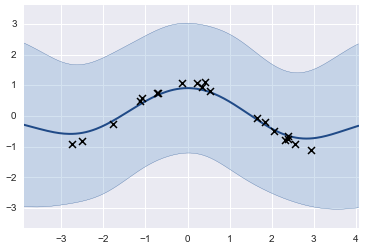
\includegraphics[width=\textwidth]{gp_cosine.png}
        \caption{Gaussian process regression}
        \label{gp}
	\end{subfigure}
    \hfill
	\begin{subfigure}[b]{0.4\textwidth}
        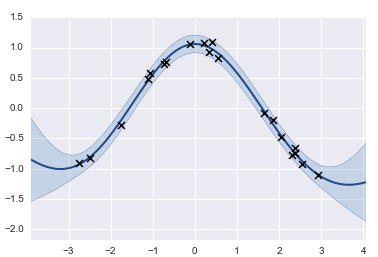
\includegraphics[width=\textwidth]{gp_cosine_optimized.png}
	    \caption{Optimized Gaussian process regression}
	    \label{gp_optimized}
	\end{subfigure}
\caption{Gaussian process regression of cosine function}
\label{gp_regression}
\end{figure}

This methodology applies for a single objective but can be extended to multiple outputs, and a sequential optimization algorithm for multi-objective problems can be implemented. This is the case for the overall project, where a sequential algorithm uses an extension of the expected improvement as the best information acquisition function (IAF)\cite{Jones2001} (applied to multiple objectives \cite{wagner2010expected}) to generate new evaluations of the experiment that is being modeled.

\section{Results}

To test the developed method, a nanoHUB tool was created, where initial observations were loaded into a Python program that executed the optimization algorithm. The tool allows an iterative process where the user can implement the experimental designs that the tool suggests, in order to input the results to the tool and continue the process of obtaining the optimal designs for the expensive experiment being studied. Also, the tool allows the experimenter to load a set of desired experimental designs to perform, in order for the algorithm to select the optimal designs to implement and to build the Pareto front from the results of the experiments. Figure \ref{tool} shows this tool, named SMOOT (Stochastic Multi-Objective Optimization Tool) after its general purpose.

\begin{figure}
\centering
    \begin{subfigure}{0.45\textwidth}
        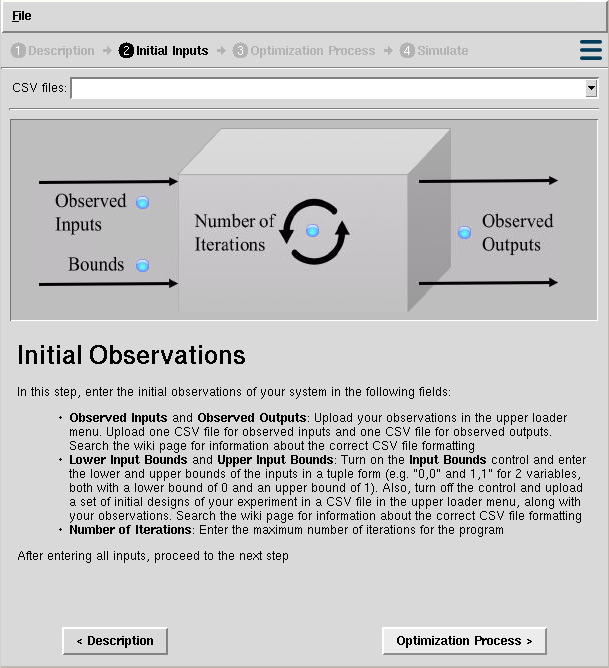
\includegraphics[width=\textwidth]{tool1}
        \caption{Interface for initial observations}
        \label{tool_1}
    \end{subfigure}
    \hfill
    \begin{subfigure}{0.45\textwidth}
        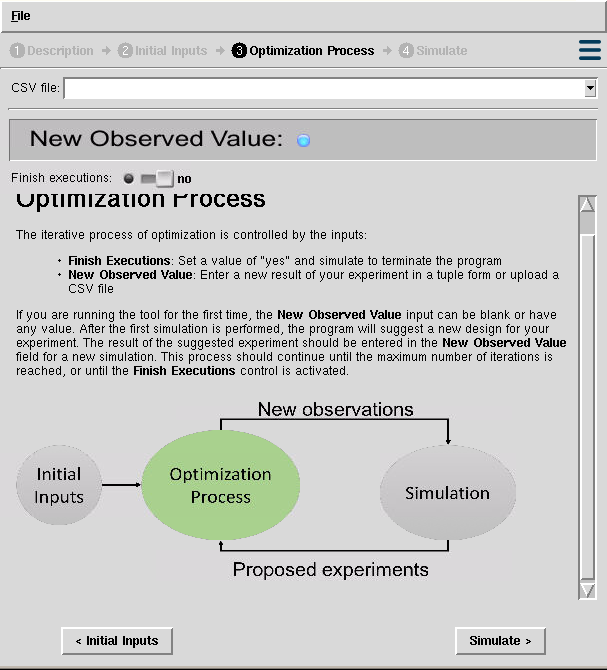
\includegraphics[width=\textwidth]{tool2}
        \caption{Interface for iterative optimization process}
        \label{tool_2}
    \end{subfigure}
\caption{SMOOT tool: a) Interface to input initial observations. b) Interface to input new results from proposed experiments}
\label{tool}
\end{figure}

\subsection{Synthetic 2-dimensional case}

As a first result, a synthetic two-dimensional function was tested in two scenarios. In both cases, the generated and ideal Pareto fronts where obtained and compared; first, with a set of 2 initial observations and 20 iterations, and then with a set of 10 initial observations and just 10 iterations.

The synthetic example describes two functions, $f_1(\vec{x})$ and $f_2(\vec{x})$ \cite{parr2013improvement}:

\begin{equation}\label{f1}
    f_1(\vec{x}) = \left( b_2 - \cfrac{5.1}{4\pi^2}b_1^2 + \cfrac{5}{\pi}b_1 - 6 \right)^2 + 10\left[ \left( 1 - \cfrac{1}{8\pi} \right)\cos(b_1) + 1 \right],
\end{equation}
\begin{multline}\label{f2}
    f_2(\vec{x}) = - \sqrt{(10.5-b_1)(b_1+5.5)(b_2+0.5)} - \cfrac{1}{30}\left( b_2 - \cfrac{5.1}{4\pi^2}b_1^2 - 6 \right)^2\\ - \cfrac{1}{3}\left[ \left( 1 - \cfrac{1}{8\pi} \right)\cos(b_1) + 1 \right],
\end{multline}

where $b_1 = 15x_1 - 5$ and $b_2 = 15x_2$. In this case, a slight modification was made to the functions in order to add noise to the input data, so that $x_1$ and $x_2$ are defined as:

\begin{align*}
    x_1 = x_1' + \epsilon\\
    x_2 = x_2' + \epsilon\\
    x_1', x_2' \in \left[0,1\right]\\
    \epsilon \sim \mathcal{N}(0,\sigma^2)
\end{align*}

\begin{figure}[!t]
\centering
    \begin{subfigure}{0.45\textwidth}
        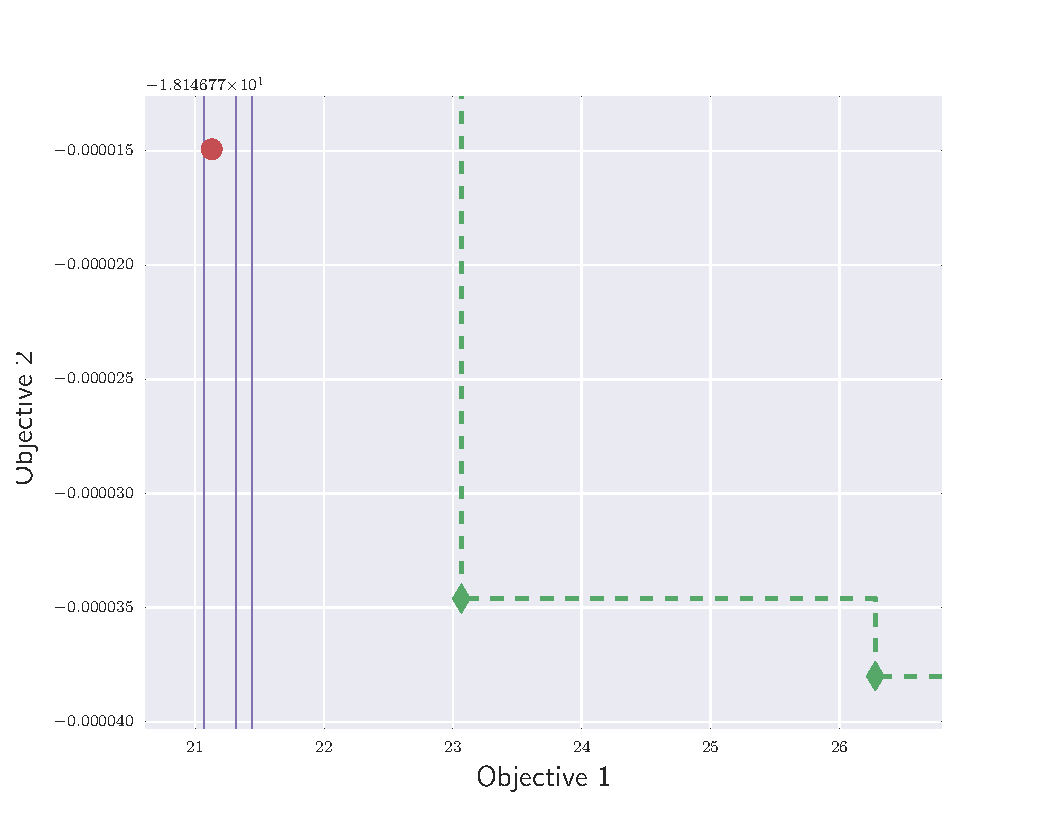
\includegraphics[width=\textwidth]{li_ex1_00}
        \caption{Initial Pareto front for 2 initial observations}
        \label{li_initial}
    \end{subfigure}
    \hfill
    \begin{subfigure}{0.45\textwidth}
        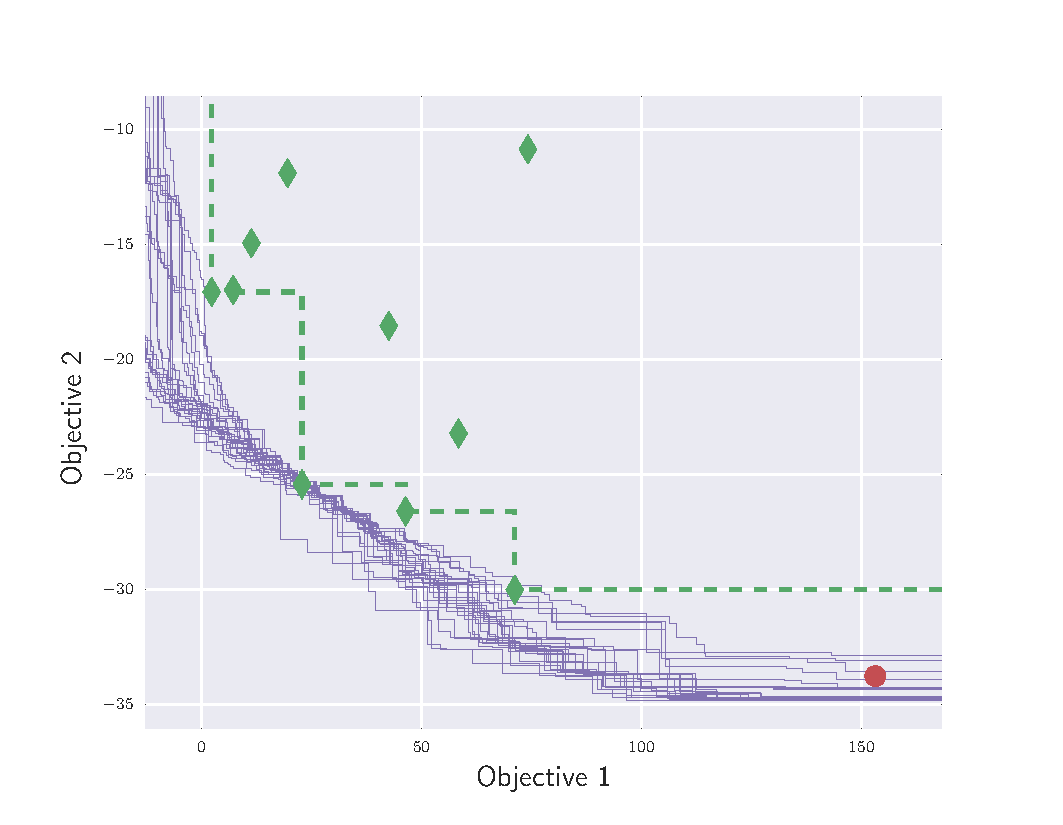
\includegraphics[width=\textwidth]{hi_ex1_00}
        \caption{Initial Pareto front for 10 initial observations}
        \label{hi_intial}
    \end{subfigure}
    \hfill
    \begin{subfigure}{0.45\textwidth}
        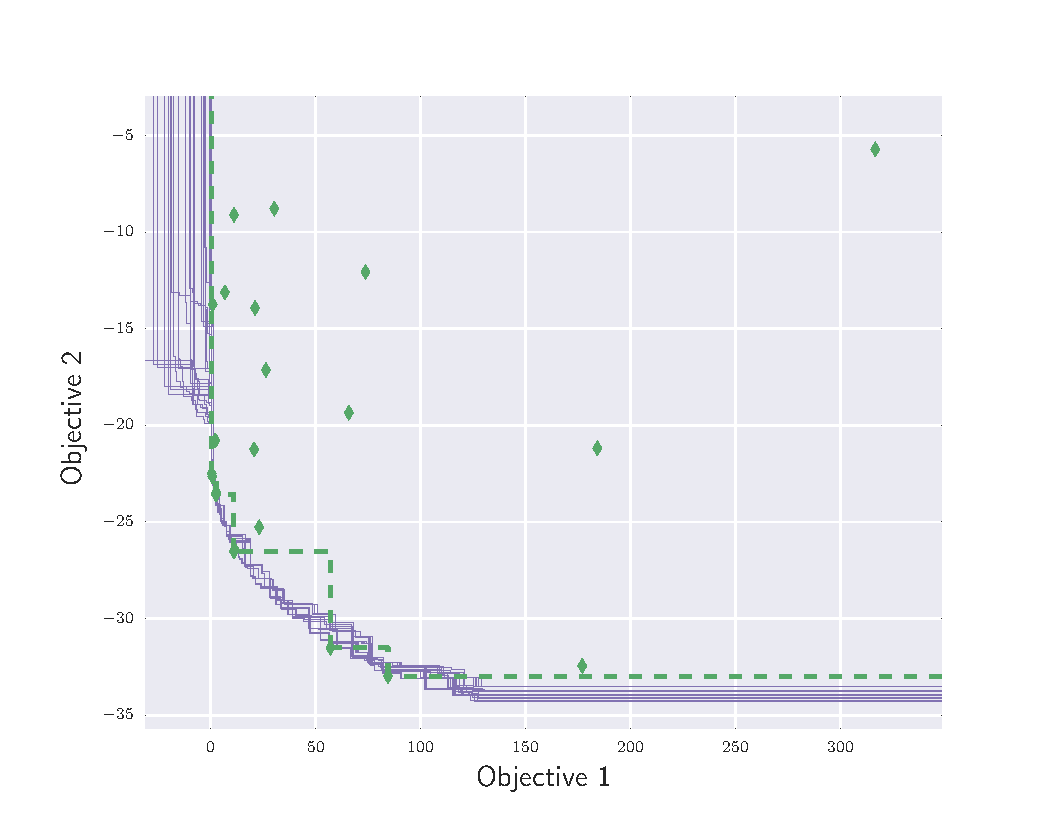
\includegraphics[width=\textwidth]{li_ex1_19}
        \caption{Final Pareto front for 2 initial observations}
        \label{li_final}
    \end{subfigure}
    \hfill
    \begin{subfigure}{0.45\textwidth}
        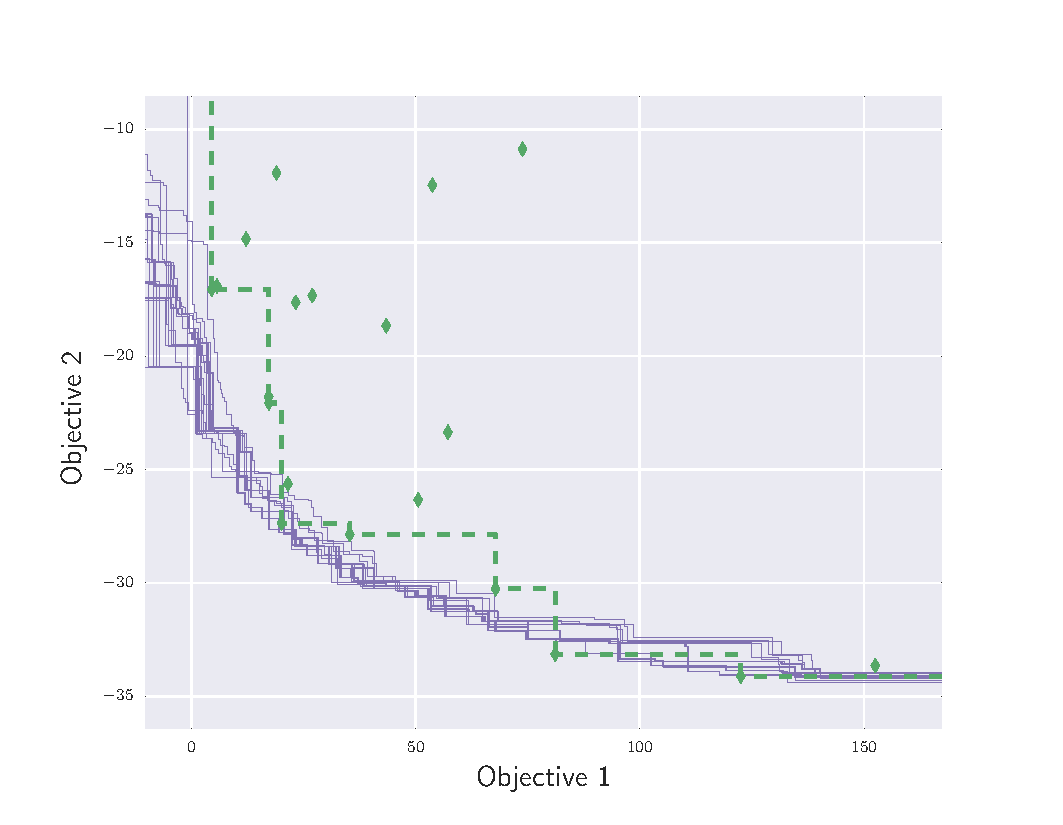
\includegraphics[width=\textwidth]{hi_ex1_09}
        \caption{Final Pareto front for 10 initial observations}
        \label{hi_final}
    \end{subfigure}
\caption{Initial Pareto fronts for the synthetic examples: a) First Pareto front with just 2 initial observations. b) First Pareto front with 10 initial observations. c) Final Pareto front with just 2 initial observations after 20 iterations. d) Final Pareto front with 10 initial observations after 10 iterations}
\label{fronts}
\end{figure}

Figure~\ref{fronts} shows the Pareto fronts for the two test cases at the first and last iteration. In the figure, the rhombus represent the points selected to be part of the front, the circled point is the point added to the front in that specific iteration and the bold line is what is estimated as the true Pareto front of the problem. Figures \ref{li_initial} and \ref{hi_intial} show the initial state of the Pareto fronts at the first iteration of both cases, and figures \ref{li_final} and \ref{hi_final} show the final state of the Pareto front after the corresponding number of iterations in both cases. To generate this plots, the two dimensional functions (\ref{f1}) and (\ref{f2}) where evaluated for every experiment proposed by the tool, produced after every iteration of the optimization algorithm. The result of the functions where introduced into the tool to continue the iterative process and obtain a new experiment proposal for the functions.

\subsection{CVD technique for graphene manufacturing}

A CVD process was studied to analyze the optimization methodology with real observations from a real experiment. The process takes place in a chamber where different gases with different concentrations turn into plasma to build graphene structures over a copper foil. In this procedure, the Raman spectrum of the foil is used to analyze vibrational properties of the layers of graphene that are deposited from the process. The G/D ratio observed in this spectrum is a variable to be maximized.

This experiment is a very expensive procedure that can't be repeated a large number of times, this is why only few observations were available and there is a certain degree of uncertainty in the input variables. Also, the process is a novel technique for manufacturing layers of graphene, so the system is treated as a black-box, as its physical behavior is not well know. This situation describes a perfect example for the usage of the methodology developed in this study.

In this example, the concentration of the different gases that are pumped inside the chamber and the pressure and power applied to the chamber constitute a set of seven input variables; and the G/D ratios of the Raman spectrum for the left and right side of the copper foil constitute a set of two output variables to be maximized. For the test case, 33 observations of different concentrations and output G/D ratios were taken, from which 15 were used as initial observations for the tool and 18 were used as experimental designs to perform. The tool selected the optimal designs from the given set of designs and the corresponding results of each experiment where given to the algorithm for the iterative process to continue. Figures \ref{cvd_pareto} and \ref{cvd_results} show the constructed Pareto front of the process and the chosen optimal outputs from the set of 33 real observations.

\begin{figure}[!t]
\centering
    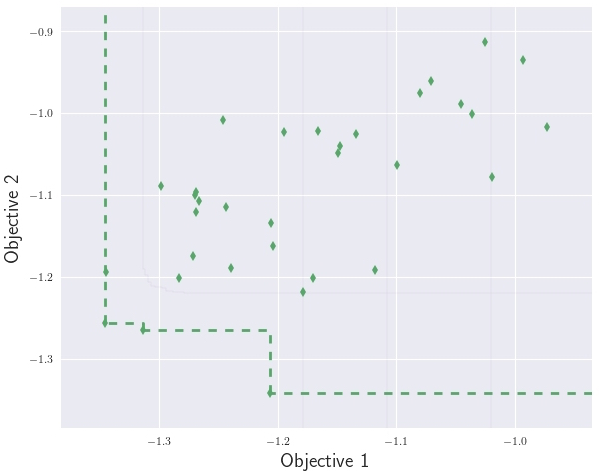
\includegraphics[width=0.6\textwidth]{ParetoFrontImage}
    \caption{Final Pareto front for the CVD process}
    \label{pareto_cvd}
\label{cvd_pareto}
\end{figure}

In figure \ref{cvd_pareto}, a set of 3 designs were chosen by the algorithm as the set of optimal experiments, whose outputs projected into the GP regressions form the Pareto front of the modeled problem showed in the graph. In this figure, the output variables had their sign inverted, as the algorithm solves a minimization problem, and a maximization of a variable can be interpreted as the minimization of the negative of the variable.

\begin{figure}[!t]
\centering
    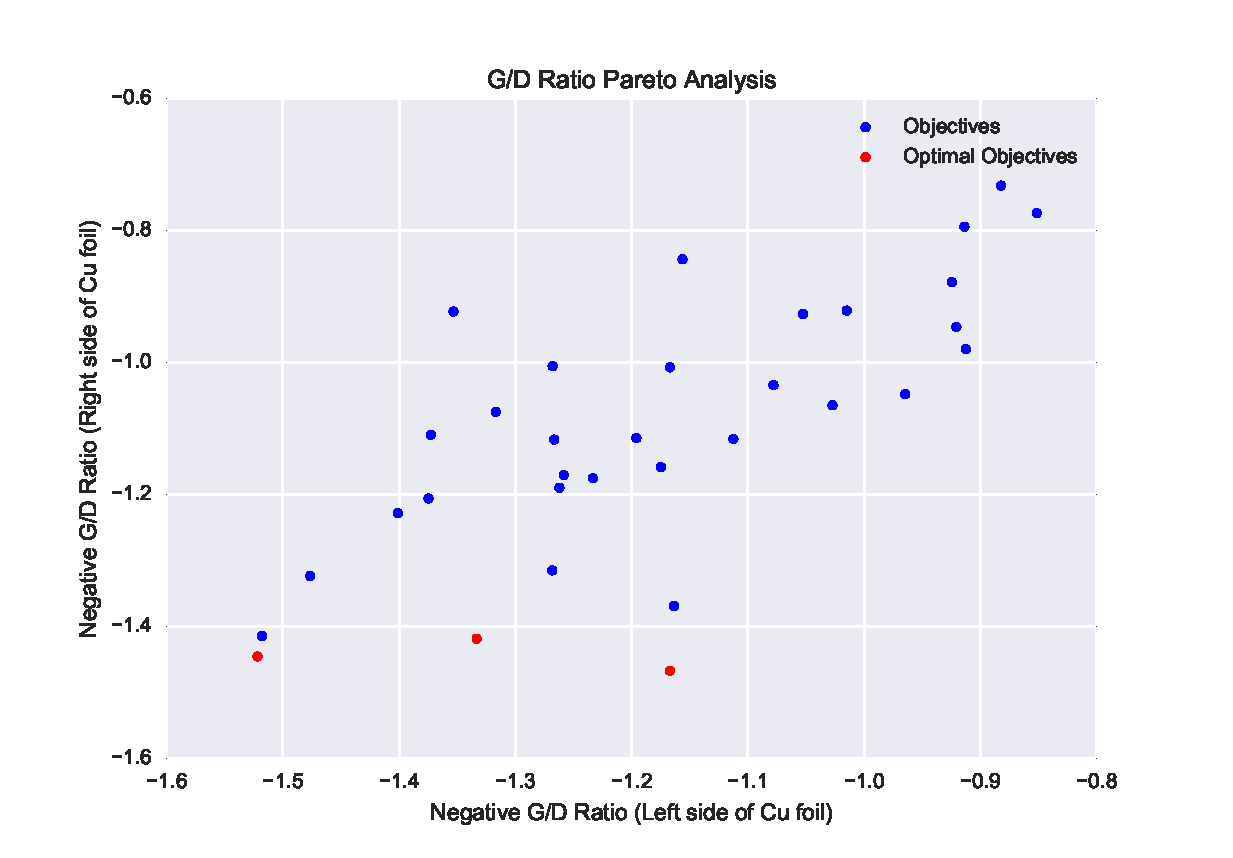
\includegraphics[width=0.8\textwidth]{Cu_foil_pareto}
    \caption{Optimal outputs for the CVD process}
    \label{optimal_cvd}
\label{cvd_results}
\end{figure}

Figure \ref{cvd_results} plots the two objectives for all the 33 observations along with the points corresponding to the 3 chosen experimental designs as the optimal designs, which corresponds to the real Pareto front in the real objective space.

\section{Discussion}

The results shown in figure \ref{fronts} demonstrate how the method is able to discover the Pareto front through an iterative process. As also shown in \cite{Huang2006}, it reinforces the usage of Gaussian process regression surrogates to extend the EGO algorithm, along with other extensions (the usage of newly developed EI due to its efficiency \cite{Jones1998}) to successfully solve the optimization problem under uncertainty.

Figure \ref{li_initial} shows how few initial observations generate a not very significant Pareto front, although its points are close to the ideal curve. On the other hand, figure \ref{hi_intial} shows that a bigger amount of observations generate a more accurate set up, as there is more information available to generate a better posterior for the surrogates of the model.

Figures \ref{li_final} and \ref{hi_final} show how the number of initial observations has a significant impact on the required number of iterations for a sufficient solution. Considering that both cases produce a similar Pareto front, the figures illustrate that few initial observations require the double amount of iterations, compared to the case of high initial data. This result can be taken as a consideration at the time of gathering initial experimental data, it can be said that more observations produce better results with less iterations. This is a consequence of the Bayesian inference used to handle the problem, as a bigger amount of information reduces uncertainty in the Gaussian process surrogates and enables more accurate models, which represent the objective functions being optimized.

This result has to be interpreted carefully, as the methodology proposed aims to solve optimization problems for expensive experiments or simulation codes, so gathering a big amount of initial observations can have a very high cost, which is contrary to the goal of this study. In this context, as long as it is reasonable, it is recommended that a high amount of initial data is entered to the tool to generate better results in a short time.

Considering the tool performance, the simulation times changed differently with every iteration, in general, for the synthetic two-dimensional example, all iterations finished with times lower than 10 minutes. This is a favorable result, as there is a high probability that the real experiment being studied for which the tool is being used can have experiments that last hours or even days.

For the case of the CVD process, figure \ref{cvd_pareto} shows a Pareto front built with 3 solutions in the objective space. As shown in the graph, the solutions dominate all of the other points and represent a correct Pareto front in the objective space built with the GP surrogates. It is interesting to note that for this case, the projected objectives of the surrogates are sparse, and it is easier to identify the set of points that dominate others.

With the 3 selected objective points and its corresponding experimental designs, the real objectives corresponding to this point were plotted along with the other 30 observations in figure \ref{optimal_cvd}. In the real objective space, it can be said that the data is sparse and has a similar behavior to the projected GP surrogates of figure \ref{cvd_pareto}, this shows that the surrogates effectively describe the data in an accurate form. Also, the selected optimal points (red points) dominate the great majority of the other points, creating a highly accurate Pareto front in the real objective space; in fact, the set of selected solutions contains the optimal value of the whole set of 33 observations, located in the lower left corner of the graph.

\section{Conclusions}

Throughout the process, the appliance of Gaussian process regressions to build surrogates for objective functions proved to be an effective choice for handling uncertainty in black box systems. The methodology was proven to be correct with synthetic and real examples, building accurate Pareto fronts for the cases where it could be constructed. This fronts showed that the Gaussian process surrogates correctly describe the objectives and enable the optimization process to be performed with uncertain data.

The GP regression surrogates proved to produce accurate predictions of data in order to perform a global optimization process, producing accurate Pareto fronts near the real know set of optimal solutions (as shown in the synthetic example of figure \ref{fronts}) and enabling the algorithm to select a set of optimal experimental designs of a real expensive experiments (as in the CVD case of figures \ref{cvd_pareto} and \ref{optimal_cvd}).

The tool created was useful in the sense that it allows experimentalists to obtain an optimal set of designs to apply in their experiments, with no extra costs or inefficient use of resources. The simulation times of the optimization algorithm are reasonable compared to the time-consuming simulation codes or experiments for whom the tool was built.

\subsubsection*{Acknowledgments}
The experimental observations of the CVD process were provided by the current graduate student Majed A. Alrefae working with Professor Timothy Fisher at the Birck Nanotechnology Center at Purdue University.

\bibliographystyle{ieeetr}
\bibliography{SURF_2016}

\end{document}
